\makeatletter
\def\input@path{{../}}
\makeatother
\documentclass[../main.tex]{subfiles}
\graphicspath{
  {"../images/02/"}
  {"./images/02/"}
}

\begin{document}
\chapter{Probability Spaces}

Probability is the best tool we currently have for predicting
future events based on past observations. To the extent that we believe physical processes are guided by certain (often hidden) equations, we can turn to probabilistic techniques to help bescribe, extrapolate and infer long-term behaviors.

Probability assumes a predictability to the world while also allowing an element of chance/noise/randomness/chaos. It describes long-term
trends and average behavior while also quantifying the extent to
which short-term behavior can be expected to deviate. While I may not
be able to predict the temperature on March 21 to within 20 degrees, I can fairly certainly predict the average for May to within 1 or 2 degrees.

Even in today's news, it has been observed that the red giant
Betelgeuse ($\alpha$-Orionis) is undergoing a precipitous decrease
in apparent brightness. Some have speculated that a supernova
is on the horizon. Data exists tracking Betelguese's magnitude
for decades so there is some precedent for concluding "this is
not normal", but the precise determination of how abnormal
this behavior is falls to the realm of probability and
statistics. There are physical laws, some of which we know,
that govern the brightness of the stars, in addition to other
unknown and perhaps unknowable factors.
\begin{figure}
	\centering
	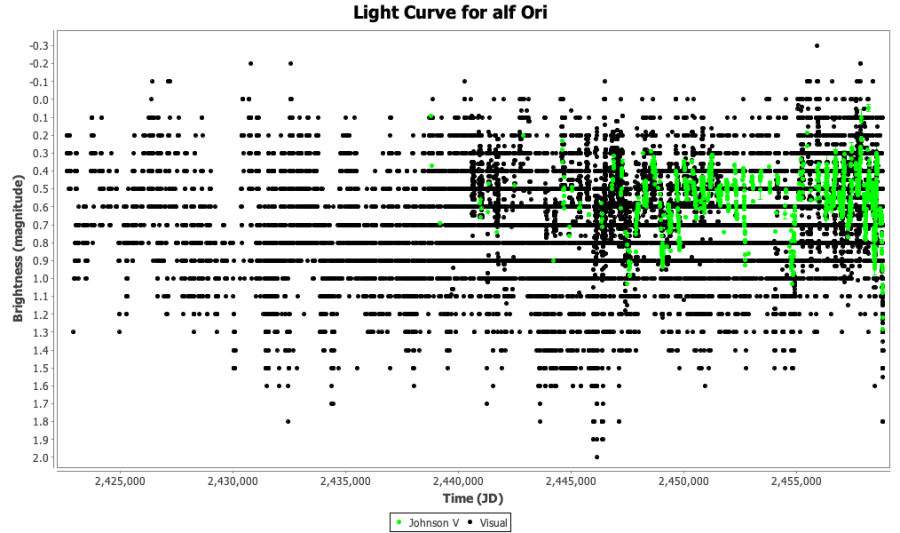
\includegraphics[width=0.7\linewidth]{alfori100yrs.png}
	\caption{Magnitude of $\alpha$-Ori, 1890-2020}
	\label{fig:alfori100yrs}
\end{figure}

The end goal of probability and statistics is to formalize a
logical method by which we can reasonably state ``given these
assumptions and these observations, I draw this conclusion,"
with a measured amount of confidence.

\section{Experiments and such}
If you flip a coin and it lands on heads, what is the probability it 
will land on heads if you flip it a second time? One-half you may say?
There are at least three reasonable answers, all different.

If you assume the coin to be fair (which was never stated and
difficult to prove), then you may believe 1/2 is the right
probability and, perhaps, no amount of evidence to the contrary would
persuade you to believe otherwise, because the statement of ``fairness"
is the one that defines your calculation.

Yet there is another method based on Bayesian Inference\footnote{which
we will study in Chapter 2} that says, ``I don't know the probability 
of heads before I flip the coin, other than it may be between 0 and 1, 
with equal probability. Since I have seen one appearance of heads,
I can calculate the probability of a second heads to be 2/3."\footnote{Never
	mind the exact calculation; we'll get to it in time.}

And a third method, called maximum likelihood estimation\footnote{covered at the end of this course}, essentially
makes the argument ``I've seen heads once, and tails never, so I
predict the coin will always land on heads" and assigns the value of
1 to the probability.

Which answer is right? Are any of them? All of them? In a sense, it
is not the job of probability to decide for you which answer is ``right." Each follows from a set of assumptions about the coin and
the world in general. Once the underlying assumptions are stated
and the goal is defined, then probability can guide us through the
calculations. 

Of course, to ascertain the true bias of the coin, one would likely try to flip it several times and count heads versus tails. Even then,
does 506 heads out of 1000 flips prove fairness? Or bias? Does 10 heads in a row indicate tails is never going to appear? Only approximate
conclusions can be drawn from these observations, but the reason we
even believe such a process to be informative is one of the assumptions underlying all of probability theory, namely that long term behaviors can
be estimated and predicted.

\subsection{Definitions}
To begin we take as undefined the terms ``procedure"
and ``outcome." Attempts to define them end up circular or
mathematically non-rigorous and add nothing to our understanding. Each
is understood as you normally understand them!

An \textbf{experiment} is defined as a procedure which results in
a specific \textbf{outcome}. Simple examples include flipping a coin, rolling three dice. More complicated are measuring the stopping distance
of a car from a certain speed, or determining the mass of a proton.

The \textbf{sample space}, sometimes denoted $\Omega$, is the set of all possible outcomes from a given experiment. We will see specific examples below.

An \textbf{event} is a subset of the sample space. It could be as small as one outcome, or as large as all of $\Omega$.

Finally, a \textbf{probability function} assigns a number $P(E)$ to
each event $E \subseteq \Omega$.

\subsection{Examples}

\begin{example}[One coin toss] Toss a fair coin. The experiment is to record which
	side lands up: heads or tails. The sample space is $\{H,T\}$.
	The probability function assigned to a \textit{fair} coin 
	would be $P(H)=P(T)=\frac12$.
\end{example}

\begin{example}[Three coin tosses]
Toss a coin three times and record which side lands up. The sample space
is $$\Omega=\{HHH, HHT, HTH, HTT, THH, THT, TTH, TTT\}.$$ Examples of \textit{events}
are `two heads', 'an odd number of tails', `more heads than tails'. One probability
function would assign 1/8 to each outcome, making the coin fair.
Another function could assign $\frac12$ to the outcome $HHH$ and $\frac{1}{16}$ to each of the other outcomes\footnote{``This
	doesn't make sense," you may protest, because if $P(HHH)=\frac12$ then $P(H)$ must be $\frac{1}{\sqrt[3]{2}}$.
	You'd be right if the flips were known to be independent, which in practice they usually are. But
	it's not strictly required for our probability function to assume independence of the 
	individual coin tosses. More on independence in a later section.}.
\end{example}

\begin{example}[Proton mass]
	Measure the mass of a proton, in grams. The sample space is, perhaps	surprisingly, all non-negative reals $\Omega=[0,\infty)$. While we all know a proton will never weigh
	1 gram, it is mathematically more pleasing to leave the upper-bound unspecified and allow the probability to fade away
	to negligible amounts, rather than abruptly stop the domain at
	some pre-determined amount. The same occurs in many applications: actuaries preparing life-expectancy tables will allow for a 
	person to live for 1000 years, with ridiculously low probability,
	just as a traffic analyst will consider equally negligible the
	case that one million cars cross an intersection during a 5\~-minute
	interval.
	
	An event in this sample space could be an interval such as
	``the mass is between $1.6726219\times10^{-24}$ and
	$1.6726220\times10^{-24}$ grams." Another event is ``the
	mass is an even number," although this event has zero probability.
\end{example}

\begin{example}[Roll two dice]
	In this experiment you roll two identical, six-sided, fair dice
	simultaneously and record the numbers that appear on the top of each\footnote{Actually you're recording the number of ``pips"
		present on the top of each die, a term I found out most
		of my students didn't know when I included it on
		a unit test in the fall term and fielded a dozen
		questions about it.}. In this example, the sample space
	depends on what you do with those two numbers. You have
	at least three choices
	\begin{enumerate}
		\item Label one die A and one B and record the numbers
		appearing on each
		\item Record the two numbers appearing, without distinguishing the two dice
		\item Record the sum of the two numbers
	\end{enumerate}

	In the first case the sample space is all ordered pairs
	$$\Omega = \{(x,y) \quad | \quad 1 \leq x,y \leq 6\}$$
	and thus has order (\textit{size}) 36. In the second case the
	sample space is \textit{unordered} pairs
	$$\Omega = \{(x,y) \quad | \quad 1 \leq x \leq y \leq 6\}$$
	where we adopt the convention of recording the smaller of the
	two results first. This space has order 21.\footnote{Add the
	${6 \choose 2}$ pairs where $x \neq y$ to the 6 pairs
	where $x=y$} 
	%
	%
	%
	Finally in the third case the sample
	space is simply the 11-element set
	$$\Omega = \{2,3,4,5,6,7,8,9,10,11,12\}$$
	
	If the die are fair then the appropriate probability functions
	to assign to each of the sample spaces are
	\begin{enumerate}
		\item $P(\omega)=\frac{1}{36}$ for all $\omega \in \Omega$
		\item $P(x,y)=
		\begin{cases}
			\frac{1}{18} & x<y\\
			 \frac{1}{36} & x=y
		\end{cases}$
		\item $P(x) = \dfrac{6-|7-x|}{36}$
	\end{enumerate}
	\end{example}

\subsection{Probability Functions}
We have seen examples of probability functions in the preceding section. Now we'll develop a rigorous definition. 

\begin{definition} Given a sample space $\Omega$, the
	\textbf{class of events} $\mathcal{F}$ is a
	class of subsets of $\Omega$ that form a \textit{sigma algebra}.
	That is, they are closed under complementation and countable union.
\end{definition}

This is a bit of a mathematical formality that we need to give a good definition of a probability function. In just about every case we encounter (if not \textit{really every} case), the class of events $\mathcal{F}$ is just the powerset of $\Omega$, that is, the set
of all subsets of $\Omega$. The important thing about sigma-algebras is the closure properties. 

\begin{definition} Given a sample space $\Omega$ and 
	an event class $\mathcal{F}$, a \textbf{probability function}
	on $\mathcal{F}$ is a function that assigns a real number to
	each element $E \in \mathcal{F}$ such that
	\begin{enumerate}
		\item $P(E) \geq 0$ for every $E \in \mathcal{F}$
		\item $P(\Omega) = 1$
		\item If $E_1, E_2, \ldots$ are disjoint sets
		in $\mathcal{F}$ then
		$$P(E_1 \cup E_2 \cup \cdots) = 
		P(E_1)+P(E_2) + \cdots$$
	\end{enumerate}
\end{definition}

Notice that nowhere in the definition do we claim that $P$ says 
anything about the ``probability" of anything occurring. That would
get us into a big mess trying to define probability in terms
of probability and also giving it a tangible interpretation. For now,
it is simply a type of function.\footnote{But we will see that
	according to provable theorems like the Law of Large Numbers,
	this definition of probability implies that it behaves like
	we want a ``probability" function to behave.}

Finally we can give a formal definition of a Probability Space.

\begin{definition}
	A \textbf{probability space} is a triple $(\Omega, \mathcal{F},
	P)$ where $\Omega$ is a set, $\mathcal{F}$ is a sigma-algebra
	of subsets of $\Omega$ and $P$ is a probability function 
	on $\mathcal{F}$
\end{definition}

\subsection{Properties of Probability Functions}
The proofs of these properties are left as an exercise.

\begin{theorem} The following properties can be proven from the above definition of a probability function. 
\begin{enumerate}
	\item $P(A^C) + P(A) = 1$ where $A^C$ is the complement of $A$, that is, everything in the set $\Omega - A$
	\item $P(\emptyset) = 0$
	\item If $A_1 \subseteq A_2$ then $P(A_1) \leq P(A_2)$
	\item $P(A_1 \cup A_2) = P(A_1) + P(A_2) - P(A_1 \cap A_2)$
\end{enumerate}
\end{theorem}

\subsection{Algebra of Sets}

\begin{theorem}[DeMorgan's Laws]
	For sets $A,B$ the following are true
	\begin{itemize}
		\item $(A \cup B)^C = A^C \cap B^C$
		\item $(A \cap B)^C = A^C \cup B^C$
	\end{itemize}
\end{theorem}

\begin{theorem}[Principle of Inclusion/Exclusion]
	$$P(A \cup B) = P(A) + P(B) - P(A \cap B)$$
	\label{thm:pie}
\end{theorem}

	\begin{figure}
	\begin{center}
		\def\firstcircle{(0,0) circle (1.5cm)}
		\def\secondcircle{(0cm:2cm) circle (1.5cm)}
		\begin{tikzpicture}
		\begin{scope}[shift={(3cm,-5cm)}, fill opacity=0.333]
		\fill[magenta] \firstcircle;
		\fill[cyan] \secondcircle;
		\end{scope}
		\begin{scope}[shift={(3cm,-5cm)}]
		\draw \firstcircle node {$A$};
		\draw \secondcircle node {$B$};
		\end{scope}
		\end{tikzpicture}
	\end{center}
	\caption{Diagram for Theorem~\ref{thm:pie}}
	\label{fig:pie}
\end{figure}

{\fontsize{10}{10}\selectfont
\subsection{Exercises}
\begin{enumerate}
	\item Verify the following relations
	\begin{enumerate}
		\item $(A \cup B)' = A'B'$
		\item $AA = A = A \cup A$
		\item $(A \cup B) - AB = AB' \cup A'B$
		\item $(A \cup B)C = AC \cup BC$
		\item $(A \cup B) - B = A - AB = AB'$
		\item $(A - AB) \cup B = A \cup B$
		\item $A' \cup B' = (AB)'$
	\end{enumerate}

	\item Find simple expressions for
	\begin{enumerate}
		\item $(A \cup B)(A \cup B')$
		\item $(A \cup B)(A' \cup B)(A \cup B')$
		\item $(A \cup B)(B \cup C)$
	\end{enumerate}

	\item State which of the following are correct and which
	are incorrect
	\begin{enumerate}
		\item $(A \cup B) - C = A \cup (B-C)$
		\item $ABC = AB(C \cup B)$
		\item $A \cup B \cup C = A \cup (B-AB) \cup (C-AC)$
		\item $A \cup B = (A-AB) \cup B$
		\item $AB \cup BC \cup CA \supset ABC$
		\item $(AB \cup BC \cup CA) \subset (A \cup B \cup C)$
		\item $(A \cup B) - A = B$
		\item $AB'C \subset A \cup B$
		\item $(A \cup B \cup C)' = A'B'C'$
		\item $(A \cup B)'C = A'C \cup B'C$
		\item $(A \cup B)'C = A'B'C$
		\item $(A \cup B)'C = C - C(A \cup B)$
	\end{enumerate}

	\item Prove Theorem 1.1
	
	\item \label{three-circles} Give an expression for $P(A \cup B \cup C)$ analogous
	to the one given for two sets in the text. (See fig~\ref{fig:three-circles})
	
	\begin{figure}
		\begin{center}
			\def\firstcircle{(0,0) circle (1.5cm)}
			\def\secondcircle{(60:2cm) circle (1.5cm)}
			\def\thirdcircle{(0:2cm) circle (1.5cm)}
			\begin{tikzpicture}
			\begin{scope}[shift={(3cm,-5cm)}, fill opacity=0.333]
			\fill[magenta] \firstcircle;
			\fill[cyan] \secondcircle;
			\fill[yellow] \thirdcircle;
			\end{scope}
			\begin{scope}[shift={(3cm,-5cm)}]
			\draw \firstcircle node[below] {$A$};
			\draw \secondcircle node [above] {$B$};
			\draw \thirdcircle node [below] {$C$};
			\end{scope}
			\end{tikzpicture}
		\end{center}
		\caption{Diagram for problem~\ref{three-circles}}
		\label{fig:three-circles}
	\end{figure}
	
\end{enumerate}
}

\section{Examples of Probability Spaces}
Before developing more theory, let's get our hands dirty with some simple examples of discrete and continuous probability spaces.

\subsection{Discrete equiprobable spaces}
These are the bread-and-butter spaces of basic probability, and, at the same time, the field admits problems that
can get quite complicated. Classic problems about rolling dice, flipping coins, pulling marbles out of bags, etc. all are examples
of discrete equiprobable spaces because the sample space of
possible outcomes is discrete and each outcome is ideally 
assumed to be equally likely. That is, if $\Omega$ contains
$n$ points, then $P(\omega) = \frac1n$ for all $\omega \in \Omega$.
Similarly if an event $E$ contains $r$ events, then $P(E) = \frac{r}{n}$.

\begin{example}
	Select a card at random from a deck of 52 cards. Let $A$
	be the event `the card is a spade' and $B$ be the event
	`the card is a face card (J,Q,K).' Compute $P(A), P(B),
	P(A \cup B), P(A \cap B)$
\end{example}

\begin{solution}
	$A$ has size 13 and $B$ has size 16. So $P(A) = \frac{13}{52},
	P(B) = \frac{12}{52}$. $A \cap B$ has 3 cards in it $\{
	J\spadesuit, Q\spadesuit, K\spadesuit\}$ so
	$P(A \cap B) = \frac{3}{52}$. Finally
	$$P(A \cup B) = P(A) + P(B) - P(A\cap B) = \frac{22}{52}$$
\end{solution}

\begin{example}
	Select two items at random from a lot containing 12 items, of which four are defective. Compute the probability that
	\begin{itemize}
		\item Neither is defective
		\item Both are defective
		\item At least one is defective
	\end{itemize}
\end{example}

\begin{solution}
	The sample space is every possible way of selecting two light bulbs from a lot of 12, namely $${12 \choose 2} = 66.$$
	\begin{itemize}
		\item Two non-defective light bulbs can be selected
		in ${8 \choose 2} = 28$ ways, giving a probability
		of $\frac{28}{66}$
		\item Two defective light bulbs can be selected in ${4
		\choose 2} = 6$ ways, giving a probability of $\frac{6}{66}$
		\item This event is the complement of "neither is defective",
		so the probability is $1-\frac{28}{66} = \frac{38}{66}$
	\end{itemize}

	It is worth pointing out at this time that this solution
	method considers an unordered sample space or, in other words,
	the light bulbs are un-labeled so the only way to distinguish
	two events is by the \textit{number} of non-defective and
	defective light bulbs and not the order in which they were
	chosen. It is possible to solve this same problem with an
	\textit{ordered} sample space, which would have size $12\cdot11 = 132$. Then the event `two defective' corresponds
	to $4 \cdot 3 = 12$ elements, giving a probability
	of $\dfrac{12}{132} = \dfrac{6}{66}$. You see that
	ordered sample spaces provide the same correct answer, as long
	as you are consistent.
\end{solution}

\begin{example}[Birthday Problem]
	In a classroom of 27 students, what is the probability
	that at least two people have the same birthday?
\end{example}

\begin{solution}
	We will ignore leap-years and determine the size of the sample
	space is the number of ways to make 27 selections from 365 days, which is $365^{27}$. (This is called selecting with repetition).
	
	Now the event `at least two are the same' is again complementary to the event `all birthdays are distinct.' To have all birthdays distinct, the first person may have any of 365 birthdays,
	the second only can be from 364 remaining days, the third
	from 363, etc. So there are 
	$$ 365 \cdot 364 \cdot 363 \cdots (365-27+1) = \dfrac{365!}{338!}
	$$ events corresponding to all birthdays distinct.
	
	So the probability of at least two birthdays the same is
	$$ P = 1 - \dfrac{365!}{338! \cdot 365^{27}} = 0.627, $$
	which is pretty good odds!
\end{solution}

\subsection{Continuous Sample Spaces}
\begin{example}
	Two points $a$ and $b$ are selected at random such that
	$b \in [-2,0]$ and $a \in [0,3]$. Find the
	probability that $|a-b| > 3$
\end{example}

\begin{solution}
	In the $ab$ plane, the sample space consists of the
	$3 \times 2$ rectangle between $(0,0)$ and $(3,-2)$.
	The event desired is the subset of points 
	for which $a-b>3$, which defines a triangle below $a-b=3$
	and inside the rectangle. The ratio of the areas gives the
	probability:  
	$$p = \dfrac{2}{6} = \dfrac{1}{3}$$
\end{solution}

\begin{example}
	A point is selected at random inside a circle. Find the probability that the point is closer to the center
	than the circumference.
\end{example}

\begin{solution}[Answer.]
	$\dfrac14$
\end{solution}

\begin{example}
	Let $X$ denote the lattice of points in the cartesian 
	plane where both co-ordinates are integers. A coin
	of diameter $\frac12$ is tossed onto the (infinite) plane.
	What is the probability that the coin covers a point in $X$?
\end{example}

\begin{solution}[Answer.]
	$\dfrac{\pi}{16}$
\end{solution}

\begin{example}
	Three points $a,b$ and $c$ are selected at random from the circumference of a circle. Find the probability that the
	points lie on a semicircle.
\end{example}

\begin{solution}[Answer.]
	$\dfrac34$
\end{solution}

\begin{example}
	A stick of unit length is broken randomly into three pieces. (Specifically, two points $a,b$ are chosen at random on the
	stick and it is cut at these two points.) What is the probability
	that the three stick pieces can be formed into a triangle?
\end{example}

\begin{solution}[Answer.]
	$\dfrac{1}{4}$. 
\end{solution}

\begin{solution}
First, consider the probability that $a < b$. By symmetry, this happens with probability $\frac{1}{2}$. 

Using the triangle inequality under this assumption gives the three relations $a < \frac{1}{2}$, $b > \frac{1}{2}$, $\frac{1}{2} > b-a$. The probability that $a$ is randomly chosen to be less than $\frac{1}{2}$ is $\frac{1}{2}$, and the probability that $b$ satisfies these constraints is $a$, so the overall probability is simply $\frac{a}{2}$. 

This next step can be made more rigorous with random variables and an expected value argument, but on average, given that $a < \frac 12$, $a$ is expected to take on the value $\frac 14$. Hence, the probability the three pieces form a triangle with $a, b$, $a < b$ is $\frac 18$. Undoing the condition gives the probability as $\frac 14$. 
\end{solution}

\section{Combinatorics Excursion}
\subsection{The Fundamental Principle of Counting}
Combinatorics is the study of counting arrangements or structures. We'll 
review just a small bit of combinatorics in the section in case the
reader needs a refresher, or perhaps a first introduction.

It begins with the following theorem about selecting items from sets
\begin{theorem}[Fundamental Principle of Counting]
	Let $A_1, A_2, \ldots, A_n$ be a collection of non-empty sets. The
	number of ways, $n$, of selecting one item from each set is equal to
	$$n = |A_1| \cdot |A_2| \cdots |A_n|$$
	\label{thm:fpc}
\end{theorem}

\begin{proof}
	Consider a tree with a root $R$, at level 0. At level 1, place
	each of the elements of $A_1$, and make each a descendant of $R$. The tree
	now has $A_1$ leaves corresponding to the ways to select one item from $A_1$. 
	Underneath each $a \in A_1$, now add a leaf at level 2 for each element in $A_2$. The tree
	now has $|A_1| \cdot |A_2|$ leaves and each leaf corresponds to a selection of two elements: one each from $A_1$ and $A_2$. Continue this process through $A_n$ and
	the $n$-level tree's leaf-count completes the proof.
\end{proof}

\begin{example}
	How many positive divisors does 720 have?
\end{example}
\begin{solution}
	720 can be factored into $720 = 2^4 \cdot 3^2 \cdot 5$. Any positive divisor $d$ must
	be of the form $2^{e_2}\cdot 3^{e_3}\cdot 5^{e_5}$ where $e_2 \in \{0,\ldots,4\}$,
	$e_3 \in \{0,1,2\}$, $e_5 \in {0,1}$. There are 30 such divisors.
\end{solution}

\subsection{Ordered samples with replacement}
Given a set of $n$ distinct elements (like numbered marbles), an
ordered selection of size $r$ with replacement corresponds to selecting
one of the $n$ elements uniformly at random, recording its value in a list,
replacing it and selecting another elements and recording its value as the 
second element in the list, and so on, until $r$ elements are listed. The list
constitutes an ordered sample. There are $n^r$ such lists, according to
the fundamental principle of counting (Theorem~\ref{thm:fpc}).
\subsection{Ordered samples without replacement}
Given a set of $n$ distinct elements (like numbered marbles), an
ordered selection of size $r$ without replacement corresponds to selecting
one of the $n$ elements uniformly at random, putting the element in a 
list and not returning it to the set, selecting a second, and so on until $r$ elements
are in the list. In this case, the fundamental principle tell us there are $n$ selections
for the first element, $(n-1)$ for the second and so on until $(n-r+1)$ for the $r$-th
element. The number of these lists is given by $n(n-1)(n-2)\cdots(n-r+1) = \dfrac{n!}{(n-r)!}$.
A common notation for this is $P^n_r$ and also $n^{\underline{r}}$.
\subsection{Unordered samples without replacement}
Unordered sampling corresponds to putting the selected elements into a
bag, or set, instead of a list. With ordered sampling, $[6,4,1]$ is distinct from $[4,6,1]$ but now
the two are the same as they both form the set $\{1,4,6\}.$ Since any set of $r$ distinct
elements can be arranged into $r!$ different lists, the number of ordered samples with replacement of size $r$ must be a factor of $r!$ larger than the number of unordered samples
with replacement. Therefore the number we seek is $
\dfrac{n^{\underline{r}}}{r!} = \dfrac{n!}{r!(n-r)!}
 = \displaystyle {n \choose r}$, the familiar binomial coefficient.
\subsection{Unordered samples with replacement}
Let's develop this idea with a specific example. Given the set ${a,b,c,d,e}$ we want
to select an unordered sample of size 12, with replacement. Since the
set is unordered we can assume it to be sorted, \textit{e.g} 
	$$(a,a,a,b,c,d,d,d,d,e,e,e).$$
This selection is equivalent to the list $(3,1,1,4,3)$, where each number counts the occurrence
of the corresponds letters in the sorted original set. Let's now describe this list
with symbols "XXX.X.X.XXXX.XXX", that is 12 X's, and 5-1=4 dots. The number of X's 
give the frequency of each letter. Now we claim that any permutation
of 12 X's and 4 dots corresponds to a list of numbers $(n_a,n_b,n_c,n_d,n_e)$
which encodes exactly one unordered sample of size 12. Furthermore this encoding is reversible
-- each sample corresponds to a string that is a permutation of "XXXXXXXXXXXX....". 
A permutation of this string is equivalent to selecting, from among 16 locations,
where the 4 dots will go, and there are $\displaystyle {16 \choose 4}$ ways to do that.

By analogy this argument can be extended easily to show the number of unordered samples with replacement from $n$ elements is given by $${n-1+r \choose n-1} = {n-1+r \choose r}$$
where the equality follows from the symmetry of the binomial coefficient.

{\fontsize{10}{10}\selectfont

\subsection{Exercises} %% taken from Ash, p.24, sec 1.4
\begin{enumerate}
	\item If a 3-digit number (000 to 999) is chosen at random, find the probability that
	exactly 1 digit will be $>5$.
	\item  Find the probability that a five-card poker hand will be:
	(a) A straight (five cards in sequence regardless of suit; ace may be high but
	not low).
	(b) Three of a kind (three cards of the same face value x, plus two cards with
	face values y and 2, with x, y, z distinct).
	(c) Two pairs (two cards of face value x, two of face value y, and one of face
	value z, with x, y, z distinct).
	\item  An urn contains 3 red, 8 yellow, and 13 green balls; another urn contains 5
	red, 7 yellow, and 6 green balls. One ball is selected from each urn. Find the
	probability that both balls will be of the same color.
	\item  An experiment consists of drawing 10 cards from an ordinary 52-card pack.
	(a) If the drawing is done with replacement, find the probability that no two
	cards will have the same face value.
	(b) If the drawing is done without replacement, find the probability that at
	least 9 cards will be of the same suit.
	\item  An urn contains 10 balls numbered from 1 to 10. Five balls are drawn without
	replacement. Find the probability that the second largest of the five numbers
	drawn will be 8.
	\item  $m$ men and $w$ women seat themselves at random in $m + w$ seats arranged in a
	row. Find the probability that all the women will be adjacent.
	\item  If a box contains 75 good light bulbs and 25 defective bulbs and 15 bulbs are
	removed, find the probability that at least one will be defective.
	\item  Eight cards are drawn without replacement from an ordinary deck. Find the
	probability of obtaining exactly three aces or exactly three kings (or both).
	\item (The game of \textit{recontre} ). An urn contains $n$ tickets numbered $1,2,...,n$.
	The tickets are shuffled thoroughly and then drawn one by one without replacement.
	If the ticket numbered $r$ appears in the $r$th drawing, this is denoted
	as a match (French: \textit{rencontre}). Show that the probability of at least one match
	is
	$$ 1 - \frac{1}{2!} + \frac{1}{3!} - \cdots + \frac{(-1)^{n-1}}{n!}
	\rightarrow 1 - e^{-1} \qquad \mbox{as } n \rightarrow \infty$$
	
	\item  A ``language" consists of three ``words," 
	$W_1 =a, W_2 = ba, W_3 = bb$. Let
	$N(k)$ be the number of ``sentences" using exactly $k$ letters (e.g., $N(1) = 1$ ($a$), $N(2) = 3,$ ($aa, ba, bb$), $N(3) =5,$ ($aaa, aba, abb, baa, bba$); no space is
	allowed between words).
	\begin{enumerate}
	\item Show that $N(k) = N(k - 1) + 2N(k - 2), k =2,3,...$ (define $N(O) =1$).
	\item Show that the general solution to the second-order homogeneous linear
	difference equation 
	[with $N(O)$ and $N(1)$ specified], is $N(k) = A2^k +
	B(-1)^k$, where $A$ and $B$ are determined by $N(O)$ and $N(1)$. Evaluate $A$
	and $B$ in the present case.
	\end{enumerate}	
\end{enumerate}
}

\subsection{Solutions to Selected Exercises} 
\begin{solution}[Solution to 1.3.6, Ex. 9]
(The game of \textit{recontre}). An urn contains $n$ tickets numbered $1,2,...,n$.
	The tickets are shuffled thoroughly and then drawn one by one without replacement.
	If the ticket numbered $r$ appears in the $r$th drawing, this is denoted
	as a match (French: \textit{rencontre}). Show that the probability of at least one match
	is
	$$ 1 - \frac{1}{2!} + \frac{1}{3!} - \cdots + \frac{(-1)^{n-1}}{n!}
	\rightarrow 1 - e^{-1} \qquad \mbox{as } n \rightarrow \infty$$
	
\end{solution}

\textbf{Remark.} This problem is known by many other names -- it is sometimes called the \textit{hat problem}, or it is the \textit{derangements} problem. 

\begin{solution}
We proceed with the Principle of Inclusion-Exclusion. 
First, consider the probability that a ticket matches. Each ticket has a probability $\frac{1}{n}$ of matching its number, and so across all $n$ tickets, we get a probability $\frac{1}{n} \cdot n = 1$. 

But wait! We've overcounted the cases where two tickets match. The probability that two given tickets will match is $\frac{1}{n(n-1)}$, which we sum over all $\binom{n}{2}$ pairs. This gives a total of $\frac{1}{2!}$ to subtract off. 

But wait once again! We've subtracted off too many times where three tickets match. This time, the probability this triplet of tickets will match is $\frac{1}{n(n-1)(n-2)}$, summed over all $\binom{n}{3}$ pairs, so we add back $\frac{1}{3!}$\ldots

Continuing on, adding back and subtracting off, we indeed get the series
\[
1 - \frac{1}{2!} + \frac{1}{3!} - \ldots + \frac{(-1)^{n-1}}{n!},
\]
which, if we let $n \to \infty$, becomes the recognizable tail of the Taylor series of $e^x$, for $x=-1$: 
\[
	\rightarrow 1 - e^{-1}.
\]

\textbf{Remark.} This gives us an insight into the \textit{Generalized Principle of Inclusion/Exclusion:}, which dictates how to find the cardinality of a union of many sets given the sizes of intersections of subsets of the sets involved, in the same adding/subtracting pattern. 

\end{solution}

\begin{solution}[Solution to 1.3.6, Ex. 10]

\end{solution}

\textbf{Remark.} This is a problem that is better suited for the Concrete Mathematics course -- in particular, one learns how to solve this latter recurrence explicitly, which we will briefly show how to do. 

\begin{solution}
We will do this with recursion. Note, of course, that any sentence of length $n$ either begins with $a$, $ba$, or $bb$. If we lop off an $a$ from the front of a word, we must be left with a sentence that has a valid length of $n-1$, and if we remove a $ba$ or $bb$ from the front of a sentence, the remaining words form a sentence of length $n-2$. In particular, \textit{any} sentence of length $n$ can be formed in this way by appending an $a$ to the front of a sentence of length $n-1$, or appending a $ba$ or $bb$ to the front of a sentence of length $n-2$. Hence, we arrive at the recurrence relation
\[
	N(k) = N(k-1) + 2N(k-2).
\]
One rigorous way to arrive at the correct explicit form of $N(k)$ is to use \textit{generating functions}, which will appear with a vengeance later in this course. We will instead appeal to a tactic more suited to a differential equations course -- i.e. using an \textit{ansatz}, or a judicious guess. 

Suppose $N(k) = r^k$ for some $r \neq 0$. If we plug $r$ into our recurrence, we get 
\[
	r^k = r^{k-1} + 2r^{k-2} \implies r^2 - r - 2 = 0.
\]
This is a very nice quadratic! In particular, this gives $r = 2, -1$. Note that any linear combination of $2^k$ and $(-1)^k$ will give a valid solution to this recurrence, so we arrive at the most general solution 
\[
	N(k) = A2^k + B(-1)^k 
\]
To solve for the coefficients $A, B$, we plug in the initial conditions $N(0) = 1, N(1) = 1$, yielding
\[
	N(k) = \frac{2}{3} \cdot 2^k + \frac{1}{3} (-1)^k.
\]
\end{solution}

\section{Conditional Probability and Independence}
\subsection{Conditional Probability}
Sometimes we are interested in the outcomes from a subset of the full sample space. 
For example maybe in a room of 100 persons, 25 of them are wearing a green shirt, while there are 65 males, of whom 15 are wearing a green shirt. Then the probability of a
randomly selected person wearing a green shirt depends on if the person is a male or not (or, if we don't know). If we don't know, then the probability is 25/100. But if
we know the person to be male, the probability becomes 15/65, which is just a bit lower.
This is the essence of \textbf{conditional probability}, in which an explicit sample (sub-)space is defined.

\begin{definition}
	Given a sample space $\Omega$ and events  $A,B \subseteq \Omega$ then
	the  \textit{conditional probability of $A$ given $B$} is defined as
	\begin{equation}
	P(A | B) = \dfrac{P(A \cap B)}{P(B)}
	\end{equation}
	\label{def:condprob}
\end{definition}

\begin{example}
	The probability of an applicant to be admitted to a certain college is 0.8.
	The probability for a student in the college to live on campus is 0.6. What
	is the probability that an applicant will be admitted to the college and will
	be assigned a dormitory housing?
\end{example}
\begin{solution}
	The probability of the applicant being admitted and receiving dormitory
	housing is defined by
	P(Accepted and Housing) = P(Housing$|$Accepted)P(Accepted)
	= (0.6)(0.8) = 0.48
\end{solution}

From the definition of conditional probability comes one of the most important
identities for intersections, namely
\begin{theorem}
	$$P(A \cap B) = P(A|B)P(B) = P(B|A)P(A)$$
\end{theorem}
\noindent
and its generalization:
\begin{theorem}
	\begin{eqnarray*}
	P(A_1 \cap A_2  \cap \cdots \cap A_n) &=&	P(A_1)P(A_2 | A_1)P(A_3 | A_2 \cap A_1) \cdots \\
	&& \qquad P(A_n | A_{n-1} \cap A_{n-2} \cap 
	\cdots \cap A_1) \\
	&=& P(A_1|A_2\cap\cdots \cap A_n)P(A_2|A_3\cap\cdots \cap A_n)\cdots \\
	&& \qquad P(A_n)
	\end{eqnarray*}
\end{theorem}

\begin{proof}
	We prove the second statement by induction. The base case is clear for $n = 2$. Suppose the statement is true for any $n$ events, and we wish the same is true for any $n+1$ events, $A_1, \ldots A_n, A_{n+1}$. Let $B = A_2 \cap \ldots \cap A_n \cap A_{n+1}$. Then, 
	\[
		P(A_1 \cap A_2 \dots \cap A_n \cap A_{n+1}) = P(A_1 \cap B) = P(A_1 | B) P(B)
	\]
	Clearly, $P(B)$ can be expanded out in the desired form via the inductive hypothesis, so we are done. 
	
	Similarly, an inductive analysis on $A_1 \cap \ldots \cap A_n$ will be sufficient for the first statement. 
\end{proof}
\noindent
A very useful form of the definition of conditional probability employs the \textbf{Law
of Total Probability}

\begin{theorem}[Law of Total Probability]
	If $C_1, \ldots, C_n$ form a partition of the sample space $\Omega$, (that is,
	the sets are mutually disjoint and their union equals $\Omega$), and $A$ is
	an event in $\Omega$ then
	\begin{equation}
	P(A) = \sum_{i=1}^n P(A|C_i)P(C_i)
	\end{equation}
\end{theorem}
\noindent
Now  Definition~\ref{def:condprob} becomes
\begin{equation}
P(B | A) = \dfrac{P(B | A)}{\sum_{i=1}^n P(A|C_i)P(C_i)}
\end{equation}

\subsection{Independence}
Given any two random processes, sometimes it is the case that the first process may affect the second; other times there is no relationship whatsoever. For example, if an individual person
rolls a die and flips a coin, there is no reason to presuppose
any effect of the first process on the second. On the other
hand if a random college student is selected and the student
is asked to state their SAT score and their family income, studies
have shown these two variables to be correlated.

Two random experiments that have no effect on each other are said to be \textit{independent}. Mathematically the definition we impose is that if two events $A,B$ are from the same sample space $\Omega$, then the outcome of one does not affect the probability of the other
\begin{definition}
	If $A,B \subseteq \Omega$ and $$P(A|B) = P(A)$$ then $A$ and $B$ are \textit{independent}
\end{definition}
\begin{corollary}
	If $A,B \subseteq \Omega$ are independent then
		\begin{equation}
		P(A \cap B) = P(A)P(B)
		\end{equation}
\end{corollary}
\begin{proof}
	$$P(A \cap B) = P(A | B)P(B) = P(A)P(B)$$ when
		$A$ and $B$ are independent. \hfill\qed
\end{proof}

\begin{example}
	Let A and B be two independent events such that $P(B| A\cup B) = \frac23$
	$
	P(A | B) = \frac12$ What is $P(B)$?
\end{example}
\begin{solution}
	$\dfrac{1}{2}$
\end{solution}

\noindent
When more than two events are considered, independence takes on some added complexity. If each pair of events are independent then we call the set of events pairwise
independent.
\begin{definition}
	Given $A_1, A_2, \ldots A_n \subseteq \Omega$, if each pair $i<j$ in $[1,\ldots,n]$
	satisfies $$P[A_1 \cap A_j] = P[A_i]P[A_j]$$ then the set of events $\{A_i\}$
	are \textbf{pairwise-independent}.
\end{definition}
\noindent
Furthermore a set of events is mutually independent if \textit{every} such intersection
can be written as a product, for all subsets of events.
\begin{definition}
	Let $\{A_{i_1}, \ldots, A_{i_k}\}$ be any subset of events in $\{A_1, \ldots A_n\}$. If every such set of size $k \geq 2$ obeys the product principle, then the
	set of events $\{A_1, \ldots A_n\}$ is said to be \textbf{mutually-independent}.
\end{definition}
\noindent
To keep things interesting, these two types of independence do not always imply each other.
\begin{example}
Consider the experiment of 
flipping two fair coins. Consider the three events:
$A$ = the first coin shows heads; $B$ = the second coin shows heads, and $C$ =
the two coins show the same result. Show that these events are pairwise
independent, but not independent.
\end{example}
{\fontsize{10}{10}\selectfont

%% Note on mutual exclusivity vs. independence -- these are NOT the same -- in particular, if events are mutually exclusive they are NOT independent
\subsection{Exercises}
\begin{enumerate}
	
	\item An urn contains 22 marbles: 10 red, 5 green, and 7 orange. You pick two at
	random without replacement. What is the probability that the first is red
	and the second is orange?
	
	\item You roll two fair dice. Find the (conditional) probability that the sum of the
	two faces is 6 given that the two dice are showing different faces.
	
	\item A machine produces small cans that are used for baked beans. The probability
	 that the can is in perfect shape is 0.9. The probability of the can having
	an unnoticeable dent is 0.02. The probability that the can is obviously dented
	is 0.08. Produced cans get passed through an automatic inspection machine,
	which is able to detect obviously dented cans and discard them. What is the
	probability that a can that gets shipped for use will be of perfect shape?
	
	\item A box of television tubes contains 20 tubes, of which five are defective. If
	three of the tubes are selected at random and removed from the box in
	succession without replacement, what is the probability that all three tubes
	are defective?
	
	\item Bowl I contains eight red balls and six blue balls. Bowl II is empty. Four
	balls are selected at random, without replacement, and transferred from bowl
	I to bowl II. One ball is then selected at random from bowl II.
	Calculate the conditional probability that two red balls and two blue balls
	were transferred from bowl I to bowl II, given that the ball selected from
	bowl II is blue.
	
	\item A machine has two parts labeled A and B: The probability that part A works
	for one year is 0.8 and the probability that part B works for one year is 0.6.
	The probability that at least one part works for one year is 0.9.
	Calculate the probability that part B works for one year, given that part A
	works for one year.
	
	\item A public health researcher examines the medical records of a group of 937
	men who died in 1999 and discovers that 210 of the men died from causes
	related to heart disease. Moreover, 312 of the 937 men had at least one
	parent who suffered from heart disease, and, of these 312 men, 102 died from
	causes related to heart disease.
	Determine the probability that a man randomly selected from this group died
	of causes related to heart disease, given that neither of his parents suffered
	from heart disease.
	
	\item An insurance company examines its pool of auto insurance customers and
	gathers the following information:
	\begin{enumerate}
		\item All customers insure at least one car.
		\item  70\% of the customers insure more than one car.
		\item  20\% of the customers insure a sports car.
		\item Of those customers who insure more than one car, 15\% insure a sports car.
	\end{enumerate}
	Calculate the probability that a randomly selected customer insures exactly
	one car and that car is not a sports car.


	\item An actuary is studying the prevalence of three health risk factors, denoted
	by $A$, $B$, and $C$ within a population of women. For each of the three factors,
	the probability is 0.1 that a woman in the population has only this risk factor
	(and no others). For any two of the three factors, the probability is 0.12 that
	she has exactly these two risk factors (but not the other). The probability
	that a woman has all three risk factors, given that she has $A$ and $B$, is 
	$\frac13$.
	What is the probability that a woman has none of the three risk factors,
	given that she does not have risk factor $A$?
	
	\item Prove that if $A$ and $B$ are independent, then so are $A$ and $B^C$.
	
	\item Prove that if $A$ and $B$ are independent, then so are $A^C$ and $B^C$.
	
	\item One urn contains 4 red balls and 6 blue balls. A second urn contains 16 red
	balls and $x$ blue balls. A single ball is drawn from each urn. The probability
	that both balls are the same color is 0.44.
	Calculate $x$.
	
	\item Assume A and B are independent events with $P(A) = 0.2$ and $P(B) = 0.3$
	Let $C$ be the event that neither $A$ nor $B$ occurs, let $D$ be the event that
	exactly one of $A$ or $B$ occurs. Find $P(C)$ and $P(D)$
	
	\item Throw a dice twice. Let A be the event the first throw came up 1, 2, or 3. Let
	B be the event that the first throw came up 3,4, or 5. Let C be the event that
	the sum of the two throws is 9. Show that $P(A \cap B \cap C) = P(A)P(B)P(C)$
	but A,B, and C are not pairwise independent.
	
	\item In a certain game of chance, a square board with area 1 is colored with sectors
	of either red or blue. A player, who cannot see the board, must specify a
	point on the board by giving an $x$-coordinate and a $y$-coordinate. The
	player wins the game if the specified point is in a blue sector. The game can
	be arranged with any number of red sectors, and the red sectors are designed
	so that
	$$R_i = \left( \dfrac{9}{20} \right) ^ i$$
	where $R_i$ is the area of the $i$th red sector.
	Calculate the minimum number of red sectors that makes the chance of a
	player winning less than 20\%.
\end{enumerate}
}

\section{Bayes' Theorem}
Bayes' Theorem can be thought of a direct corollary of the definitions and theorems we already have. Recall our definition for conditional probability on two events $A$ and $B$, written both ways:
\[
	P(B|A) = \frac{P(A\cap B)}{P(A)} \quad P(A|B) = \frac{P(A\cap B)}{P(B)}
\]
We can thus find equivalent expressions for $P(A \cap B)$ --
\[
	P(B|A) P(A) = P(A|B) P(B),
\]
and thus we have
\begin{theorem}[Bayes' Theorem]
\[P(A|B) = \frac{P(B|A) P(A)}{P(B)} \]
\end{theorem}
This is often used to ``flip'' the direction of the conditionality. If we know something about $P(B|A)$, we are able to infer something about $P(A|B)$ given that we know information about $P(A)$ and $P(B)$. 

In deep learning, Bayes' Theorem can also be interpreted in another way. If we know $P(A)$, and we can find out $P(B)$, we can recompute and thus ``learn'' $P(A|B)$. For example, if we believe something about an underlying probability distribution, such as believing a die is fair,  and we learn new data about that distribution, we can update what our beliefs are about that probability distribution based on our empirical results. 

If $P(B)$ is not directly computable, we can use the Law of Total Probability: 
\begin{corollary}
If $A_1, \ldots A_n$ is a partition of the sample space $\Omega$, then 
\[
	P(A_k|B) = \frac{P(B|A_k) P(A_k)}{\sum_{i=1}^n P(B|A_i) P(A_i)}
\]
\end{corollary}

We can use this to do an exercise from the previous section: 
\begin{solution}[Alt. solution to Sec. 1.4.3, Ex. 6] %% fix this
Let event $A_i$ be the probability $i$ blue marbles are drawn and put into the second bucket, and $B$ the probability a blue marble is then drawn from the second bucket. By Bayes' Theorem,
\[
	P(A_2|B) = \frac{P(B|A_2) P(A_2)}{\sum_{i=1}^4 (B|A_i) P(A_i)}
\]
How is this easier to compute? Note that $P(A_i)$ can be easily computed: 
\[
	P(A_i) = \frac{\dbinom{8}{4-i} \dbinom{6}{i}}{\dbinom{14}{4}}
\]
In general, $P(B|A_i)$ is also easily computed -- if $i$ blue marbles are put into the second bucket, then clearly the probability is $\frac{i}{4}$. 

We can now easily compute the numerator: 
\[
	P(B|A_2) P(A_2) = \frac{2}{4} \cdot \frac{\dbinom{8}{2} \dbinom{6}{2}}{\dbinom{14}{4}}
\]
We now condition the numerator over all the terms in the denominator. Note that every factor in the denominator has this $\binom{14}{4}$  term, so we neglect it. This gives us the answer we had before for this problem: 
\[
	P(A_2|B) = \frac{\frac{2}{4}\tbinom{8}{2} \tbinom{6}{2}}{\frac{0}{4}\tbinom{8}{4} \tbinom{6}{0} + \frac{1}{4}\tbinom{8}{3} \tbinom{6}{1} + \frac{2}{4}\tbinom{8}{2} \tbinom{6}{2} + \frac{3}{4}\tbinom{8}{1} \tbinom{6}{3} + \frac{4}{4}\tbinom{8}{0} \tbinom{6}{4}} = \frac{70}{173} = 0.4895
\]
\end{solution}
Let's look at another example:
\begin{example}[Car Insurance, 10.2]


An auto insurance company insures drivers of all ages. An actuary compiled
the following statistics on the company’s insured drivers:

\begin{center}
	
\begin{tabular}{|p{0.5in}|p{0.8in}|p{1.5in}|}

	\hline
	Age of
Driver
& Probability
of Accident & 	Portion of Company’s
Insured Drivers
\\
	\hline
	16-20 & 0.06 & 0.08 \\
	21-30 & 0.03 & 0.15 \\
	31-65 & 0.02 & 0.49 \\
	66-99 & 0.04 & 0.28 \\
	\hline
\end{tabular}

\end{center}
A randomly selected driver that the company insures has an accident. Calculate the probability that the driver was age 16-20.
\end{example}
\begin{solution}
$\dfrac{16}{101} = 0.158$
\end{solution}

\begin{example}[Hospital, 10.4]
	\noindent
	Upon arrival at a hospital’s emergency room, patients are categorized ac-
	cording to their condition as critical, serious, or stable. In the past year:
	\begin{enumerate}[label=(\alph*)]
	\setlength{\itemsep}{-0.5em}
	\item 10\% of the emergency room patients were critical;
	 \item 30\% of the emergency room patients were serious;
	\item the rest of the emergency room patients were stable;
	\item 40\% of the critical patients died;
	\item 10\% of the serious patients died; and
	\item 1\% of the stable patients died.
	\end{enumerate}
	Given that a patient survived, what is the probability that the patient was
	categorized as serious upon arrival?
\end{example}
\begin{solution}
$\dfrac{45}{154} = 0.292$
\end{solution}

Bayes' theorem also gives us a more cautious analysis on medical tests. Generally, if we believe a test has a $95\%$ chance of correctly identifying whether a given person has the disease, we'd think that's a pretty decent test! Not necessarily, says Bayes' Theorem\ldots

Let's define a few terms to describe how ``good'' a test is. For a test, its \textbf{specificity} is the ratio of its true positives to the total number of positives it gives -- i.e. it measures how good a test is at finding positives. A test's \textbf{sensitivity} is the the ratio of the test's true negatives to the total number of negatives -- i.e. it measures how good a test is at finding negatives.

With this in mind, consider the following: 
\begin{example}[Disease, 10.7]
A blood test indicates the presence of a particular disease 95\% of the time
when the disease is actually present. The same test indicates the presence of
the disease 0.5\% of the time when the disease is not present. One percent of
the population actually has the disease.
Calculate the probability that a person has the disease given that the test
indicates the presence of the disease.
\end{example}
\begin{solution}
	$\dfrac{190}{289} = 0.657$
\end{solution}

%If Dr. White has a miracle test for a disease and has 100\% specificity, this test \textit{looks} great, the 
\begin{example}
A variant: for the above test, is it possible that we can improve probability one has the disease given that they get a positive test result to be greater than 90\%? 
\end{example}

\begin{solution}
No! Even if the test is able to perfectly identify true positives (i.e. its specificity is 100\%), we still won't achieve the desired 90\% cutoff line. 
\end{solution}
% ans: NO! 
Here is a final example on posterior/prior probabilities, and updating our beliefs on a probability distribution based on new data: 
\begin{example} % posterior/prior distribution. 
Consider a six-sided die, but the side labeled ``1'' might have been changed to any number from 1-6. Assume the die is still fair, and assume that the probability of changing the 1 to any of $1-6$ is also even. Find the probability distribution of the unknown side given that the die comes up as 6 on its first roll. 

More mathematically, find $P(\text{1 changed to k}|\text{roll a 6})$ for all $k = 1, 2, \ldots 6$. 
\end{example}

\begin{solution}
$\dfrac{1}{7}$ for $k = 1, 2, 3, 4, 5$, $\dfrac{2}{7}$ for $k = 6$. 
\end{solution}

% \begin{solution} 
% %% show computation
% \end{solution}

Notice that having been provided with this additional information, we have to update our initial assumption based this result.  


\end{document}
